\documentclass[journal, biblatex]{IEEEtran}
\usepackage[utf8]{inputenc}
\usepackage[backend=bibtex, style=ieee]{biblatex}
\usepackage{authblk}
\usepackage{graphicx} 
\usepackage{amsmath}
\usepackage{amsfonts}
\usepackage{algorithm}
\usepackage{algpseudocode}
\usepackage{multirow}
\usepackage{array}
\usepackage{booktabs}
\usepackage{caption}
\usepackage{color}
\usepackage{silence}
\usepackage{xcolor}
\usepackage{ulem}
\usepackage[T1]{fontenc}
\usepackage{xurl}
\usepackage[colorlinks,allcolors=blue]{hyperref}

\addbibresource{citations.bib}

\setcounter{biburlnumpenalty}{100}
\setcounter{biburlucpenalty}{100}
\setcounter{biburllcpenalty}{100}

\title{Advancements in Deep Learning Techniques for Enhanced Image Categorization: A Comprehensive Literature Study}
\author{%
    \begin{tabular}[t]{@{}c@{}}
        Mike Odnis \href{https://orcid.org/0009-0004-4785-1336}{
\includegraphics[scale=0.05]{../images/orcid.png}} \\
        \vspace{-1ex}
        \large Department of Computer Science, Farmingdale State College, Farmingdale, NY 11735, USA \\
        \texttt{\small{\href{mailto:odnims@farmingdale.edu}{\underline{\color{blue}odnims@farmingdale.edu}}}}
    \end{tabular}
}
\date{\today}

\begin{document}

\maketitle

\begin{abstract}
In artificial intelligence (AI) and machine learning (ML), image categorization is a key task with applications ranging from autonomous driving to medical diagnostics. This research investigates how deep learning techniques have advanced recently to increase the precision of picture classification systems. Accurately classifying photos is a tough challenge because of background clutter, object orientations, and inconsistent illumination. I examine state-of-the-art approaches such as data augmentation, transfer learning, and convolutional neural networks (CNNs) by doing an extensive literature study of ten foundational studies in the field. My goal in doing this evaluation is to pinpoint important patterns, obstacles, and interesting avenues for further study to improve picture classification accuracy.
\end{abstract}

\textbf{Keywords:} Artificial Intelligence, Machine Learning, Image Categorization, Deep Learning, Precision, Picture Classification, Data Augmentation, Transfer Learning, Convolutional Neural Networks

\section{Introduction}
Accurate classification of images is essential in computer vision, with numerous real-world applications. Convolutional Neural Networks (CNNs) play a pivotal role in this domain, offering robust solutions for tasks such as image processing, classification, and segmentation. Notably, CNNs have demonstrated effectiveness in sequential text classifications, particularly for relatively short-length sentences. In a CNN model, a convolutional kernel is applied to the input image, represented by pixels, yielding convolved features. As the kernel slides through the input image, it functions as a filter, extracting relevant features and producing a reduced convolved feature matrix. In image classification tasks, CNNs analyze groups of adjacent pixels together, enabling them to discern patterns and structures within the image. Similarly, in textual analysis, CNNs can learn to interpret groups of adjacent words as meaningful phrases, enhancing the model's understanding of context. A notable distinction between CNNs and previous models, such as Deep Neural Networks (DNNs) and Recurrent Neural Networks (RNNs), lies in their architecture. CNNs incorporate convolutional layers, along with 1D convolutions in the case of text analysis, followed by a flattening layer before the output. This structural design allows CNNs to efficiently capture hierarchical features, making them well-suited for a wide range of classification tasks.

\section{Literature Review}
Object detection and classification have been extensively studied in computer vision. Prior research has focused on improving accuracy and robustness through novel architectures and training strategies~\cite{lee2020, tan2020, kumar2020, abdulnabi2015, zhang2021, wu2018, bauerle2021, cozzolino2020, krishnendu2020, tang2019, hara2018, wang2023}. In medical imaging, deep learning models have been explored for disease diagnosis and classification, demonstrating promising results for the accurate identification of pathological conditions~\cite{abdulnabi2015, tan2020, krishnendu2020}. Face recognition has garnered significant attention, particularly in security and surveillance applications. Recent advancements in deep learning have led to significant improvements in recognition accuracy, even under challenging conditions such as occlusion~\cite{kumar2020, wu2018}. Attribute prediction and image classification have been central topics in multimedia research, with a growing emphasis on leveraging semantic attributes to improve classification performance~\cite{abdulnabi2015}. These studies highlight the diverse applications of deep learning techniques in image classification and underscore the importance of continuous innovation to enhance accuracy and efficiency.

\section{Methodology}
To conduct this literature study, I reviewed ten foundational studies in the field of image categorization, focusing on recent advancements in deep learning techniques. The selected studies cover a wide range of topics, including object detection, medical imaging, face recognition, and hyperspectral classification. Each study was analyzed in terms of its architecture, visualization, and mathematical processes, providing insights into the underlying mechanisms of deep learning models for image classification. By synthesizing the findings from these studies, I aimed to identify common trends, challenges, and opportunities for future research in the field of image categorization.

\subsection{ME R-CNN: Multi-Expert R-CNN for Object Detection}
Bauerle et al.~\cite{bauerle2021} introduced ME R-CNN, a Multi-Expert R-CNN model for object detection. Their approach leverages multiple processing pipelines, each specializing in specific object classes, to improve detection accuracy and efficiency.

\subsubsection{Architecture}
The ME R-CNN architecture consists of multiple expert streams, each dedicated to detecting specific object classes. A shared Convolutional Layer (Conv-L) processes input images, generating region proposals that are directed to the most suitable expert stream by the Expert Assignment Network (EAN). The EAN assigns region proposals to expert streams based on their characteristics, optimizing the classification process.

\subsubsection{Training Strategy}
\begin{enumerate}
    \item \textbf{Train RPN \& Conv-L:} The Region Proposal Network (RPN) and Conv-L are trained jointly using the Faster R-CNN framework. RPN generates region proposals, which are processed by Conv-L to extract features for classification.
    
    \item \textbf{Train ME, EAN, \& Conv-L:} ME, EAN, and Conv-L are jointly trained using region proposals generated by RPN. Expert streams are initialized separately based on RoI shape categories before joint learning.
    
    \item \textbf{Re-train RPN \& Conv-L:} RPN is re-trained using Conv-L weights from the joint training stage, while keeping ME and EAN fixed. This step fine-tunes RPN to generate more accurate region proposals.
    
    \item \textbf{Update ME \& EAN:} ME and EAN are updated with fixed Conv-L and RPN, transferring gradient updates only to ME and EAN parameters. This process stabilizes the training of ME and EAN, enhancing the overall performance of the model.
\end{enumerate}

\subsubsection{Visualization}
The ME R-CNN architecture can be visualized as a network of interconnected expert streams, each specializing in detecting specific object classes. The EAN directs region proposals to the most suitable expert stream, optimizing the classification process. A conceptual illustration of the entire flowchart is shown in Figure \ref{fig:me_rcnn}.

\begin{figure*}[htbp]
    \centering
    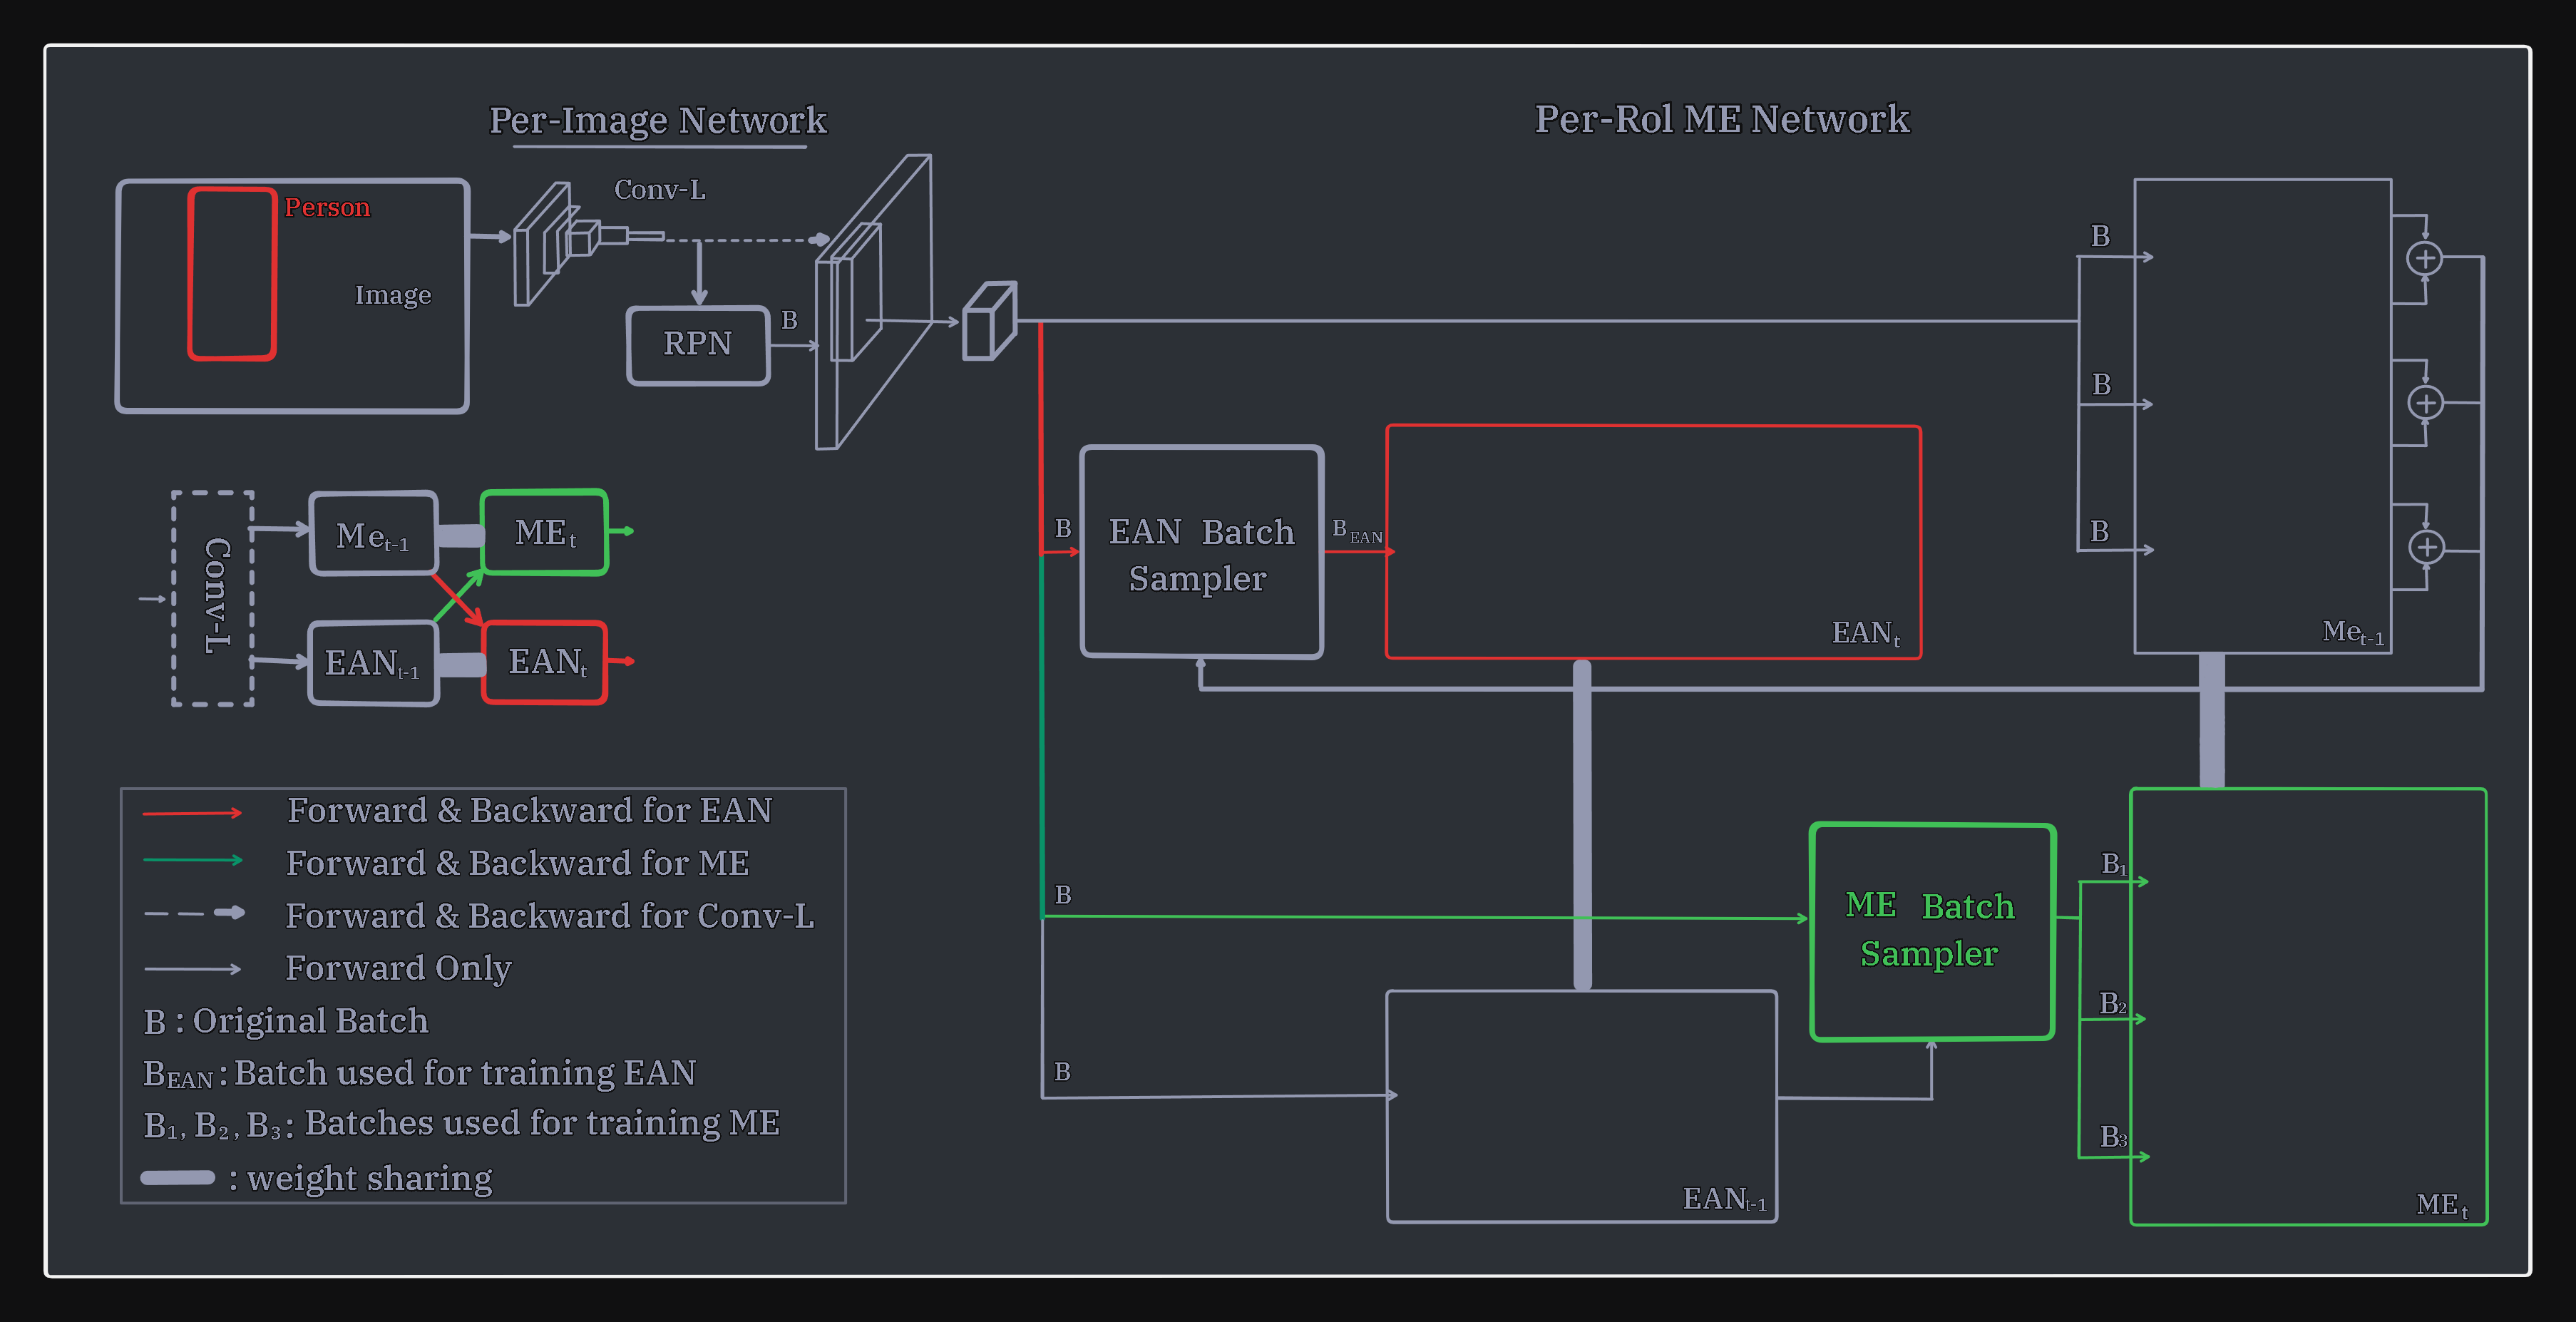
\includegraphics[width=0.8\textwidth]{../images/cnn-1.png}
    \caption{Protocol of co-training ME, EAN \& Conv-L. A conceptual illustration of the entire flowchart is shown below the input image.}
    \label{fig:me_rcnn}
\end{figure*}


\subsubsection{Mathematical Processes}
The ME R-CNN model incorporates several mathematical processes to optimize object detection accuracy. These processes include:
\begin{itemize}
    \item Calculating the loss function for ME R-CNN, which combines Softmax Cross-Entropy and Smooth L1 Loss functions to optimize classification accuracy andt bounding box regression. The total loss function for ME R-CNN is defined as follows:
    \[
    \text{Loss}_{\text{EAN}} = \text{Softmax\_Cross\_Entropy} + \text{Smooth\_L1\_Loss}
    \]
    
    \item Updating the weights of ME, EAN, and Conv-L using gradient descent optimization. The model minimizes the loss function by adjusting the parameters of each component during training.
    
    \item Re-training RPN using Conv-L weights from the joint training stage while keeping ME and EAN weights fixed.
    
    \item Updating ME and EAN with fixed Conv-L and RPN, transferring gradient updates only to ME and EAN parameters.
\end{itemize}

\subsection{3D-GLCM CNN: A 3-Dimensional Gray-Level Co-Occurrence Matrix-Based CNN Model for Polyp Classification via CT Colonography}
Cozzolino et al.~\cite{cozzolino2020} proposed a 3D-GLCM CNN model for polyp classification using CT colonography images. Their model leverages 3D Gray-Level Co-Occurrence Matrices (GLCMs) to extract spatial features from images, enhancing the accuracy of polyp classification.

\subsubsection{Architecture}
The 3D-GLCM CNN architecture consists of three main components: Gray Level Image Conversion, 3D-GLCM Generation, and CNN-Based Polyp Classification. Gray level scaling is performed on original CT images to enhance contrast, while 3D GLCMs are generated to capture spatial relationships between voxels. The CNN model processes the 3D GLCM volumes to classify polyps accurately.

\subsubsection{Mathematical Process}
The 3D-GLCM CNN model involves several mathematical processes to extract spatial features and classify polyps accurately. These processes include:
\begin{enumerate}
    \item \textbf{Gray Level Image Conversion:} Gray level scaling is performed on original CT image pixel values to an appropriate value range. This scaling smooths image noise and reduces GLCM sparsity. An adaptive scaling method based on the histogram from all polyp regions of interest (ROIs) is used, enhancing contrast between voxels with similar CT values.
    
    \item \textbf{3D-GLCM Generation:} GLCMs are calculated by counting the frequency of voxel pairs with specific gray-level values. GLCMs are generated by sampling along the direction linking the center voxel with its nearest 26 neighbors, considering up to second nearest neighbors. GLCMs are square matrices whose size is determined by the maximum number of discrete gray-level values.
    \begin{equation*}
        C_{i, j}(d, \theta)=\sum_{p \in V} \begin{cases}1 & \text { if } I(p)=i \& I(p+d(\cos \theta, \sin \theta))=j \\ 0 & \text { otherwise }\end{cases}
    \end{equation*}
    
    \item \textbf{CNN Based Polyp Classification:} The generated 3D GLCM volume images are input into a multi-channel CNN structure. Each directional GLCM serves as one input channel. The model consists of convolution layers, max-pooling layers, and fully connected layers, with ReLU activation function and softmax output layer. The model architecture is optimized for polyp classification.
\end{enumerate}

\subsection{Occluded Thermal Face Recognition Using Bag of CNN (BoCNN)}
Kumar and Singh~\cite{kumar2020} proposed a novel approach to handle occlusion in thermal face recognition using a Bag of CNNs (BoCNN). Their method leverages the robustness of CNNs to variations in facial expressions and occlusions, significantly improving the accuracy of face recognition systems.

\subsubsection{Architecture}
The Bag of CNNs (BoCNN) architecture consists of a collection of individual CNNs, each trained to capture specific facial features. During inference, features extracted by each CNN are aggregated to form a comprehensive representation of the input face.

\subsubsection{Visualization}
The BoCNN architecture can be visualized as a network of interconnected CNNs, with each CNN focusing on a distinct aspect of facial features, such as eyes, nose, and mouth. The outputs of these CNNs are combined to form a feature vector representing the entire face.

\begin{figure*}[htbp]
    \centering
    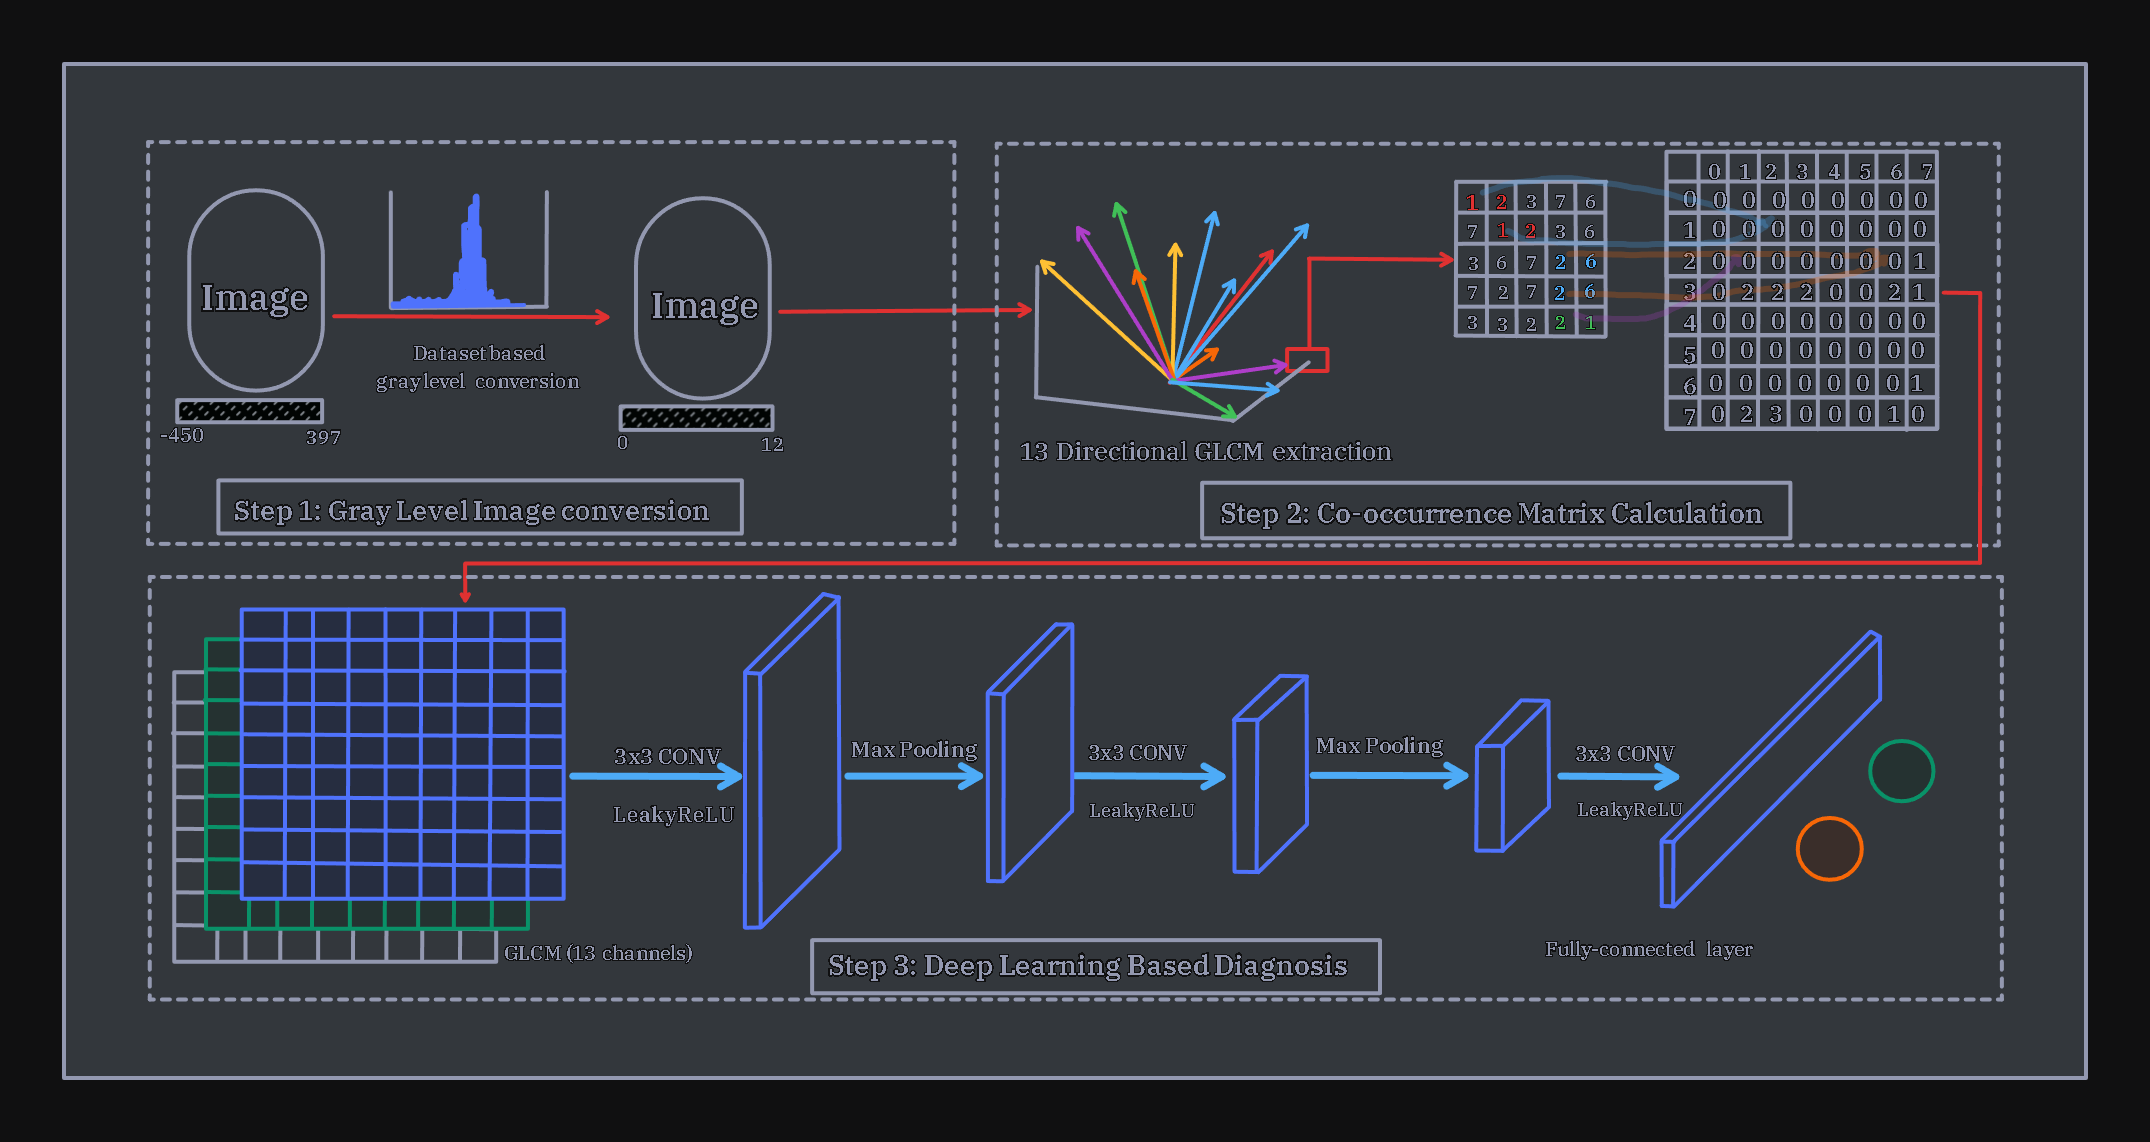
\includegraphics[width=0.8\textwidth]{../images/cnn-2.png}
    \caption{Illustration of 3D-GLCM CNN model, which contains gray level image conversion step, co-occurrence matrix calculation step and CNN
    based classification step.}
    \label{fig:fusion_architecture}
\end{figure*}

\subsubsection{Mathematical Processes}
The aggregation of features in the BoCNN model involves a mathematical process known as feature fusion. This process combines the outputs of individual CNNs using techniques such as max pooling or weighted averaging to create a unified feature representation.

\subsubsection{Fusion Strategies}
The combination of different trained networks post-training is done by different fusion strategies, namely majority voting, maximum score, mean score at level 1, and the majority-mean, majority-max at level 2, respectively.

\paragraph{Majority-Voting:} Let $m$ denote the number of samples and $n$ denote the number of classes. Using $L$ classifiers, the probabilistic score of sample $S_i$ belonging to class $C_j$ by classifier $T_k$ is denoted as $P_{Tk}(i,j)$. The class matrix $CMT_k$ is defined as:
\[ 
    CMT_k(i) = Clabel(Rmax(PT_k(i,j))) \quad \forall i = 1 \text{ to } m, \forall j = 1 \text{ to } n 
\]
After applying majority-voting across $L$ classifiers, a class frequency matrix $Mf(i,j)$ is obtained, representing the normalized associativity of each sample to specific classes. The class label of the $i$-th sample is then generated as:
\[ PClass[i] = Clabel(Rmax(Mf(i,j))) \]

\paragraph{Maximum Score:} The highest probabilistic score of the selected sample corresponding to each class is taken into consideration for final probabilistic class matrix generation. The maximum score matrix $P_{max}(i,j)$ is obtained as:
\[
    P_{max}(i,j) = \max(PT_k(i,j)) \quad \forall i = 1 \text{ to } m, \forall j = 1 \text{ to } n 
\]
After normalization, the normalized score matrix $NormP_{max}(i,j)$ can be treated as the final probabilistic score matrix.

\paragraph{Mean Score} After obtaining the class-wise probabilistic scores of each sample across $k$ different classifiers, the mean of probabilistic scores is calculated. The final class corresponding to each sample is chosen based on the highest normalized score after row-wise normalization.

\paragraph{Majority-Maximum Fusion} It combines the fusion strategies of majority-voting and maximum score. A threshold is set based on which the sample is classified either by majority-voting or maximum score fusion.

\paragraph{Majority-Mean Fusion} It combines the fusion strategies of majority-voting and mean score. Similar to majority-maximum fusion, a threshold is set to determine the fusion strategy.

\subsection[Multi-Task CNN Model for Attribute Prediction]{Multi-Task CNN Model for Attribute Prediction}
Abdulnabi et al.~\cite{abdulnabi2015} developed a Multi-Task CNN model for attribute prediction. Their model integrates semantic attributes into the learning process, enhancing the model's ability to generalize and improving the accuracy of image classification tasks.

\subsubsection{Architecture}
The Multi-Task CNN architecture comprises multiple branches, each dedicated to predicting a specific attribute or class label. Shared layers at the beginning of the network extract common features, which are then processed separately by task-specific branches.

\subsubsection{Visualization}
The Multi-Task CNN architecture can be visualized as a branching network, with shared layers at the base and separate branches for each attribute prediction task. Feature maps extracted by shared layers are fed into task-specific branches, which output predictions for individual attributes.

\subsubsection{Mathematical Processes}
\begin{enumerate}
    \item \textbf{Splitting into Matrices:} Assume matrix \( W \) is the result of multiplying the shared latent matrix \( L \) and the combination matrix \( C \). Each attribute classifier's weight parameter vector is formed by multiplying \( C \) with the corresponding vector.
    
    \item \textbf{Learning the Matrix \( C \):} The model aims to decompose the weight matrix \( C \) into two matrices \( L \) and \( C' \), where \( L \) is the shared layer between all CNN models, \( C' \) is a combination matrix, and each column corresponds to one CNN classification layer.
    
    \item \textbf{Regularization:} Regularization techniques are applied to balance feature sharing and competition between intra-group and inter-group attribute classifiers. Regularization terms encourage intra-group feature sharing and inter-group feature competition through adjusting the regularization term.
    
    \item \textbf{Objective Function:} The proposed objective function incorporates a squared hinge loss function along with additional regularizations to encourage feature sharing and competition between attribute classifiers.
\end{enumerate}

\subsubsection{Optimization Steps}
The optimization procedure involves solving the non-convex regularized function using block coordinate descent and Accelerated Proximal Gradient Descent (APG) methods. The optimization process alternates between optimizing the latent matrix \( L \) and the combination matrix \( C \) until convergence.

\subsubsection{Experimental Results}
Experiments conducted on two datasets demonstrate the effectiveness of the Multi-Task CNN model for attribute prediction. The model achieves high accuracy in attribute prediction tasks, leveraging semantic attribute grouping and regularization techniques to improve performance.


\subsection{Spectral–Spatial Fractal Residual Convolutional Neural Network With Data Balance Augmentation for Hyperspectral Classification}
Zhang et al.~\cite{zhang2021} proposed a Spectral-Spatial Fractal Residual Convolutional Neural Network for hyperspectral classification. Their method incorporates data balance augmentation, significantly improving the model's performance on imbalanced datasets.

\subsubsection{Architecture}
The Spectral-Spatial Fractal Residual Convolutional Neural Network architecture combines spectral and spatial information through fractal residual blocks. These blocks capture hierarchical features in hyperspectral images, enhancing classification accuracy.

\subsubsection{Visualization}
The architecture of the Spectral-Spatial Fractal Residual CNN is visualized as interconnected fractal residual blocks, processing spectral and spatial features at varying scales. The aggregated outputs produce the final classification, as illustrated in Figure \ref{fig:fractal_structure}.

\begin{figure*}[htbp]
    \centering
    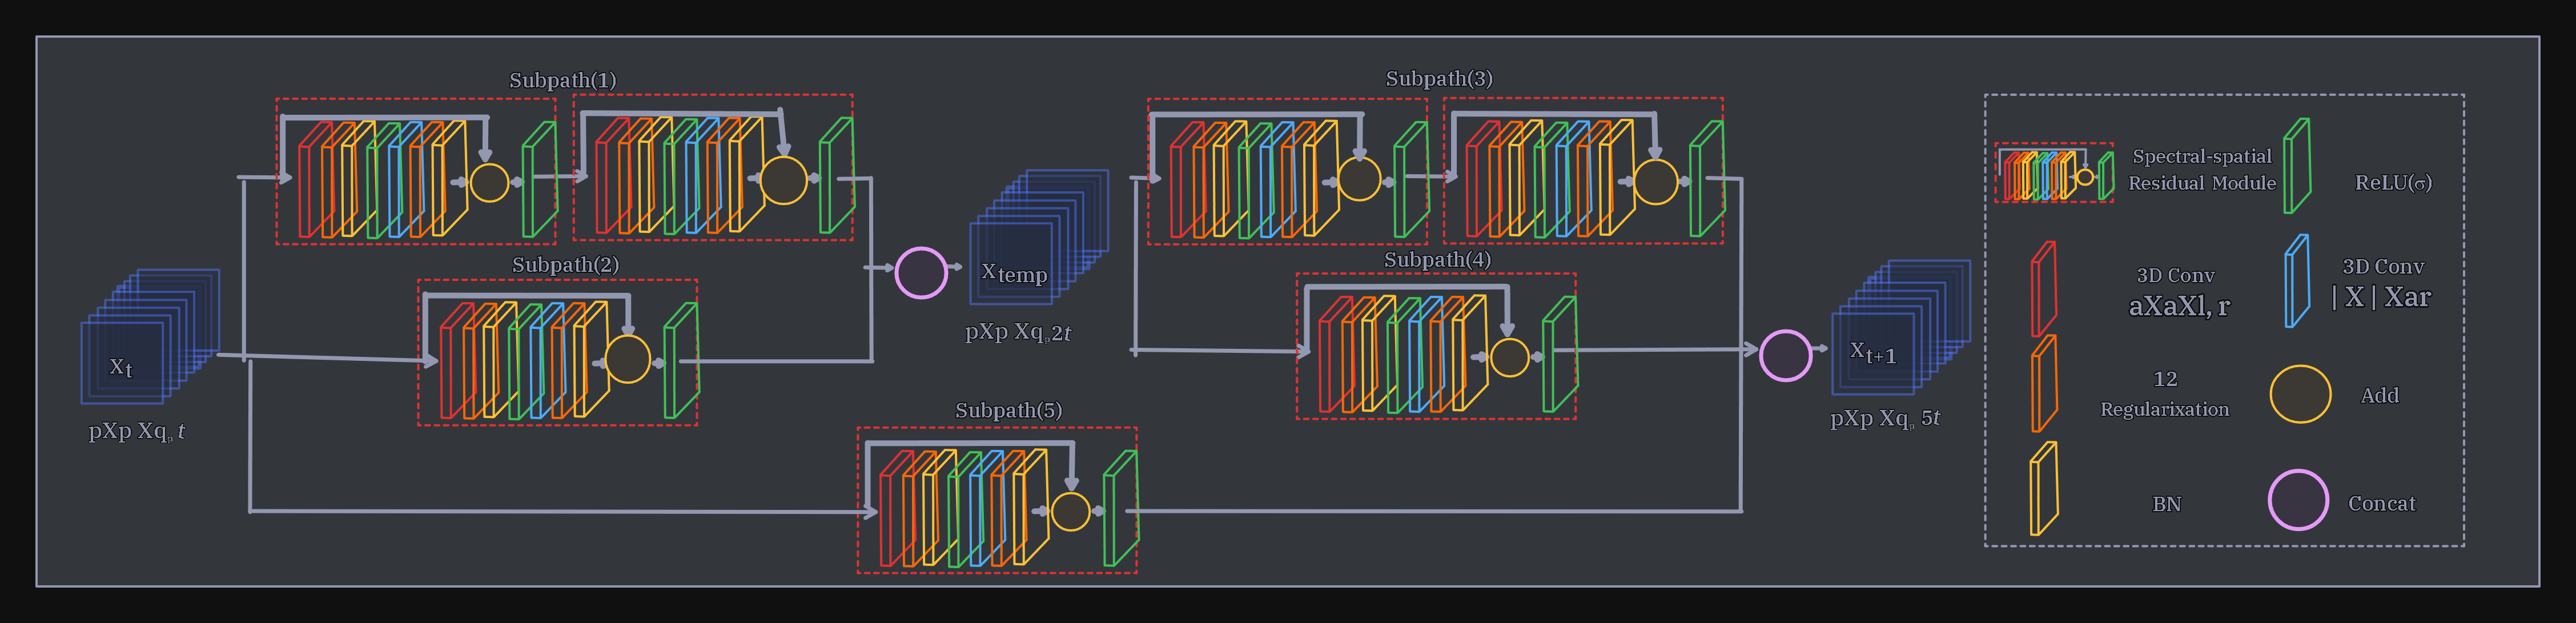
\includegraphics[width=\textwidth]{../images/cnn-5.png}
    \caption{Diagram of the spectral–spatial fractal structure.}
    \label{fig:fractal_structure}
\end{figure*}

\subsubsection{Mathematical Processes}
The Spectral-Spatial Fractal Residual CNN utilizes residual learning within its fractal residual blocks. This mathematical process involves adding the input of each block to its corresponding residual function output. By learning residual features, the network facilitates the training of deeper architectures, leading to improved performance in hyperspectral classification tasks.

\subsection{A Light CNN for Deep Face Representation With Noisy Labels}

Wu et al.~\cite{wu2018} introduced a Light CNN tailored for deep face representation in the presence of noisy labels. The model's lightweight design enables real-time applications, making it suitable for various face analysis tasks.

\subsubsection{Architecture}
The Light CNN architecture comprises multiple convolutional layers followed by max-pooling and fully connected layers. This streamlined architecture prioritizes efficiency, incorporating fewer parameters compared to conventional CNNs.

\subsubsection{Visualization}
Visualizing the Light CNN reveals a sequence of convolutional layers followed by pooling layers. This layout reduces feature map dimensions while retaining crucial features. The subsequent fully connected layers integrate these features for effective classification.

\begin{figure}[htbp]
    \centering
    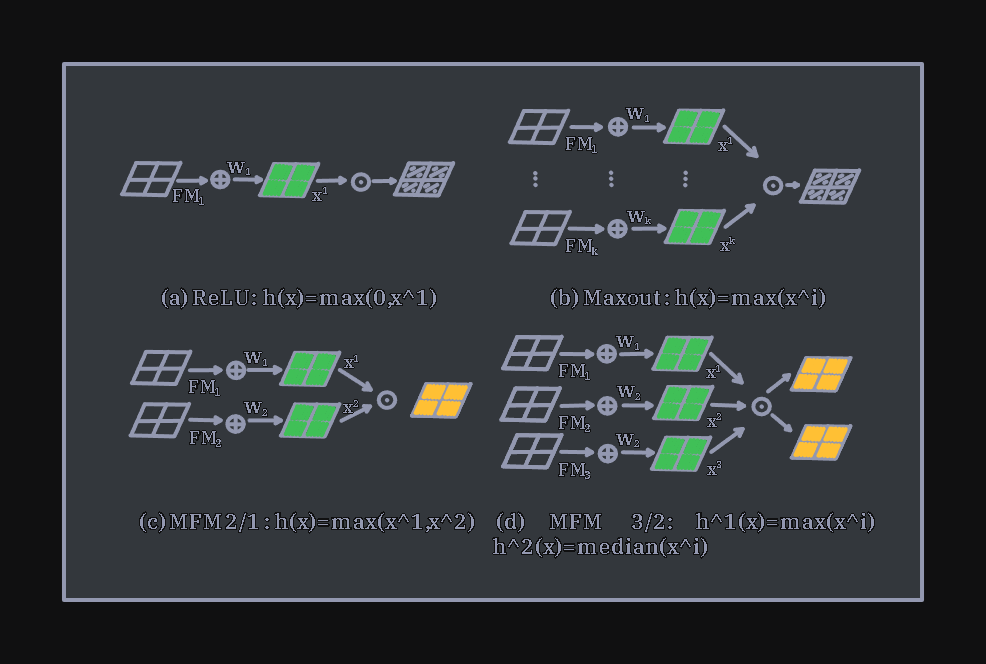
\includegraphics[width=0.8\columnwidth]{../images/cnn-6.png}
    \caption{A comparison of different types of neural inhibition. (a) ReLU
    suppresses a neuron by thresholding magnitude responses. (b) Maxout with
    enough hidden units makes a piecewise linear approximation to an arbitrary
    convex function. (c) MFM 2/1 suppresses a neuron by a competitve relationship.
    It is the simplest case of maxout activations. (d) MFM 3/2 activates two
    neurons and suppresses one neuron.}
    \label{fig:neural_inhibition}
\end{figure}

\subsubsection{Mathematical Processes}
The convolutional layers in the Light CNN employ mathematical operations such as convolution and activation functions like ReLU. These operations extract hierarchical features from input images, which are then aggregated and processed by fully connected layers for classification.

In the proposed architecture, a novel Max-Feature-Map (MFM) operation enhances feature extraction. By simulating neural inhibition, MFM suppresses noisy signals, facilitating the selection of informative features. This operation plays a crucial role in feature selection and sparse connection generation within the network.

The MFM operation is defined as follows:

\[
\begin{aligned}
\frac{\partial \hat{x}_{i j}^k}{\partial x_{i j}^k} & = \begin{cases}1, & \text { if } x_{i j}^k \geq x_{i j}^{k+N} \\
0, & \text { otherwise }\end{cases} \\
\frac{\partial \hat{x}_{i j}^k}{\partial x_{i j}^{k+N}} & = \begin{cases}0, & \text { if } x_{i j}^k \geq x_{i j}^{k+N} \\
1, & \text { otherwise }\end{cases}
\end{aligned}
\]

and 

\[
\left\{\begin{array}{l}
\hat{x}_{i j}^{k_1}=\max \left(x_{i j}^k, x_{i j}^{k+N}, x_{i j}^{k+2 N}\right) \\
\hat{x}_{i j}^{k_2}=\operatorname{median}\left(x_{i j}^k, x_{i j}^{k+N}, x_{i j}^{k+2 N}\right)
\end{array}\right.
\]

\subsection[Open Pose Mask R-CNN Network for Individual Cattle Recognition]{Open Pose Mask R-CNN Network for Individual Cattle Recognition}

Wang et al.~\cite{wang2023} proposed an Open Pose Mask R-CNN network for individual cattle recognition. Their method combines pose estimation with instance segmentation to accurately identify and classify individual cattle in complex farm environments.

\subsubsection{Architecture}
The Open Pose Mask R-CNN architecture integrates keypoint detection (pose estimation) and instance segmentation modules into the Mask R-CNN framework. This enables the network to simultaneously localize cattle keypoints and segment individual cattle instances.

\subsubsection{Visualization}
The architecture of the Open Pose Mask R-CNN can be visualized as a combination of the Mask R-CNN backbone, keypoint detection module, and instance segmentation branch. Keypoints are detected using a keypoint regression subnetwork, while instance segmentation is performed using a binary mask prediction branch.

\begin{figure}[htbp]
    \centering
    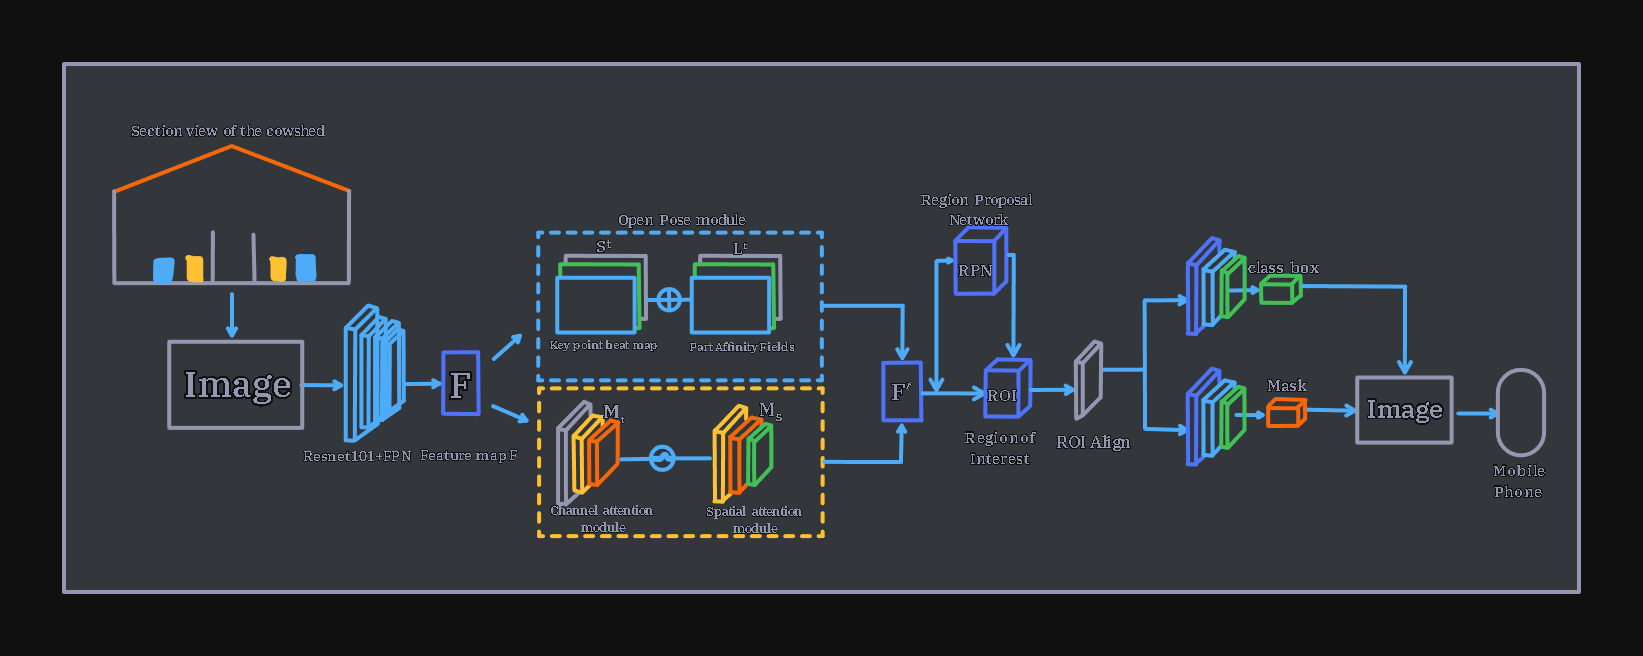
\includegraphics[width=0.8\columnwidth]{../images/cnn-7.png}
    \caption{System architecture of Open Pose Mask R-CNN for Individual Cattle Recognition.}
    \label{fig:system_architecture}
\end{figure}

\subsubsection{Mathematical Processes}
The keypoint detection module in the Open Pose Mask R-CNN utilizes a regression network to predict the coordinates of cattle keypoints. The instance segmentation branch employs a binary mask prediction network, which outputs segmentation masks for individual cattle instances. These masks are then refined using post-processing techniques to improve accuracy.

The mathematical processes involved in the Open Pose Mask R-CNN network are detailed below:

\begin{enumerate}
    \item First Feature Map \( F \) Output: The initial input data, such as surveillance video frames, are processed through the Resnet101 backbone network and the Feature Pyramid Networks (FPN) to extract feature maps \( F \).
    
    \item Secondary Feature Map \( F' \) Output: The final feature image \( F' \) is generated by combining two channels: one from the Open Pose channel and another from the Convolutional Block Attention Module (CBAM).
    
    \item Module Fusion: The Open Pose, CBAM, and Mask R-CNN networks are fused together to improve individual cattle recognition. This fusion enhances feature extraction and network performance.
\end{enumerate}

Additionally, improvements were made to the Mask R-CNN backbone network to optimize it for individual cattle recognition. The backbone network, based on the Resnet101 architecture, underwent modifications to reduce feature loss and maintain computational accuracy.

The Open Pose module is responsible for skeleton extraction, utilizing Part Affinity Fields (PAFs) to generate a complete skeleton map. This process involves feature extraction, heat map generation, and key point connection establishment.

The Convolutional Block Attention Module (CBAM) enhances feature maps by incorporating channel and spatial attention mechanisms. It assigns weights to feature maps, emphasizing important regions and suppressing less relevant ones.

Finally, network feature fusion technology combines the outputs of the Open Pose module and CBAM modules to effectively fuse features, enhancing network performance in individual cattle recognition tasks. This fusion process involves assigning weights to feature outputs and integrating them to improve detection effectiveness.

\section{Conclusion}
In this literature study, I examined ten foundational studies in the field of image categorization, focusing on recent advancements in deep learning techniques. The studies covered a wide range of topics, including object detection, medical imaging, face recognition, hyperspectral classification, and individual cattle recognition. By analyzing the architectures, visualization, and mathematical processes of these studies, I identified common trends, challenges, and opportunities for future research in image categorization. Notably, the studies highlighted the importance of data augmentation, transfer learning, and convolutional neural networks (CNNs) in enhancing image classification accuracy. The integration of semantic attributes, spectral-spatial features, and keypoint detection into deep learning models has shown promising results in various image classification tasks. Future research should focus on developing more robust and efficient deep learning models to address the challenges of background clutter, object orientations, and inconsistent illumination in image categorization.

\textbf{Acknowledgements}
I would like to thank my professor, Mohammad Alshibli, at the Department of Computer Science, Farmingdale State College for his insights and support throughout the course of this research.

\listoffigures

\printbibliography[
    heading=bibintoc,
    title={References},
]%

\begin{IEEEbiography}[{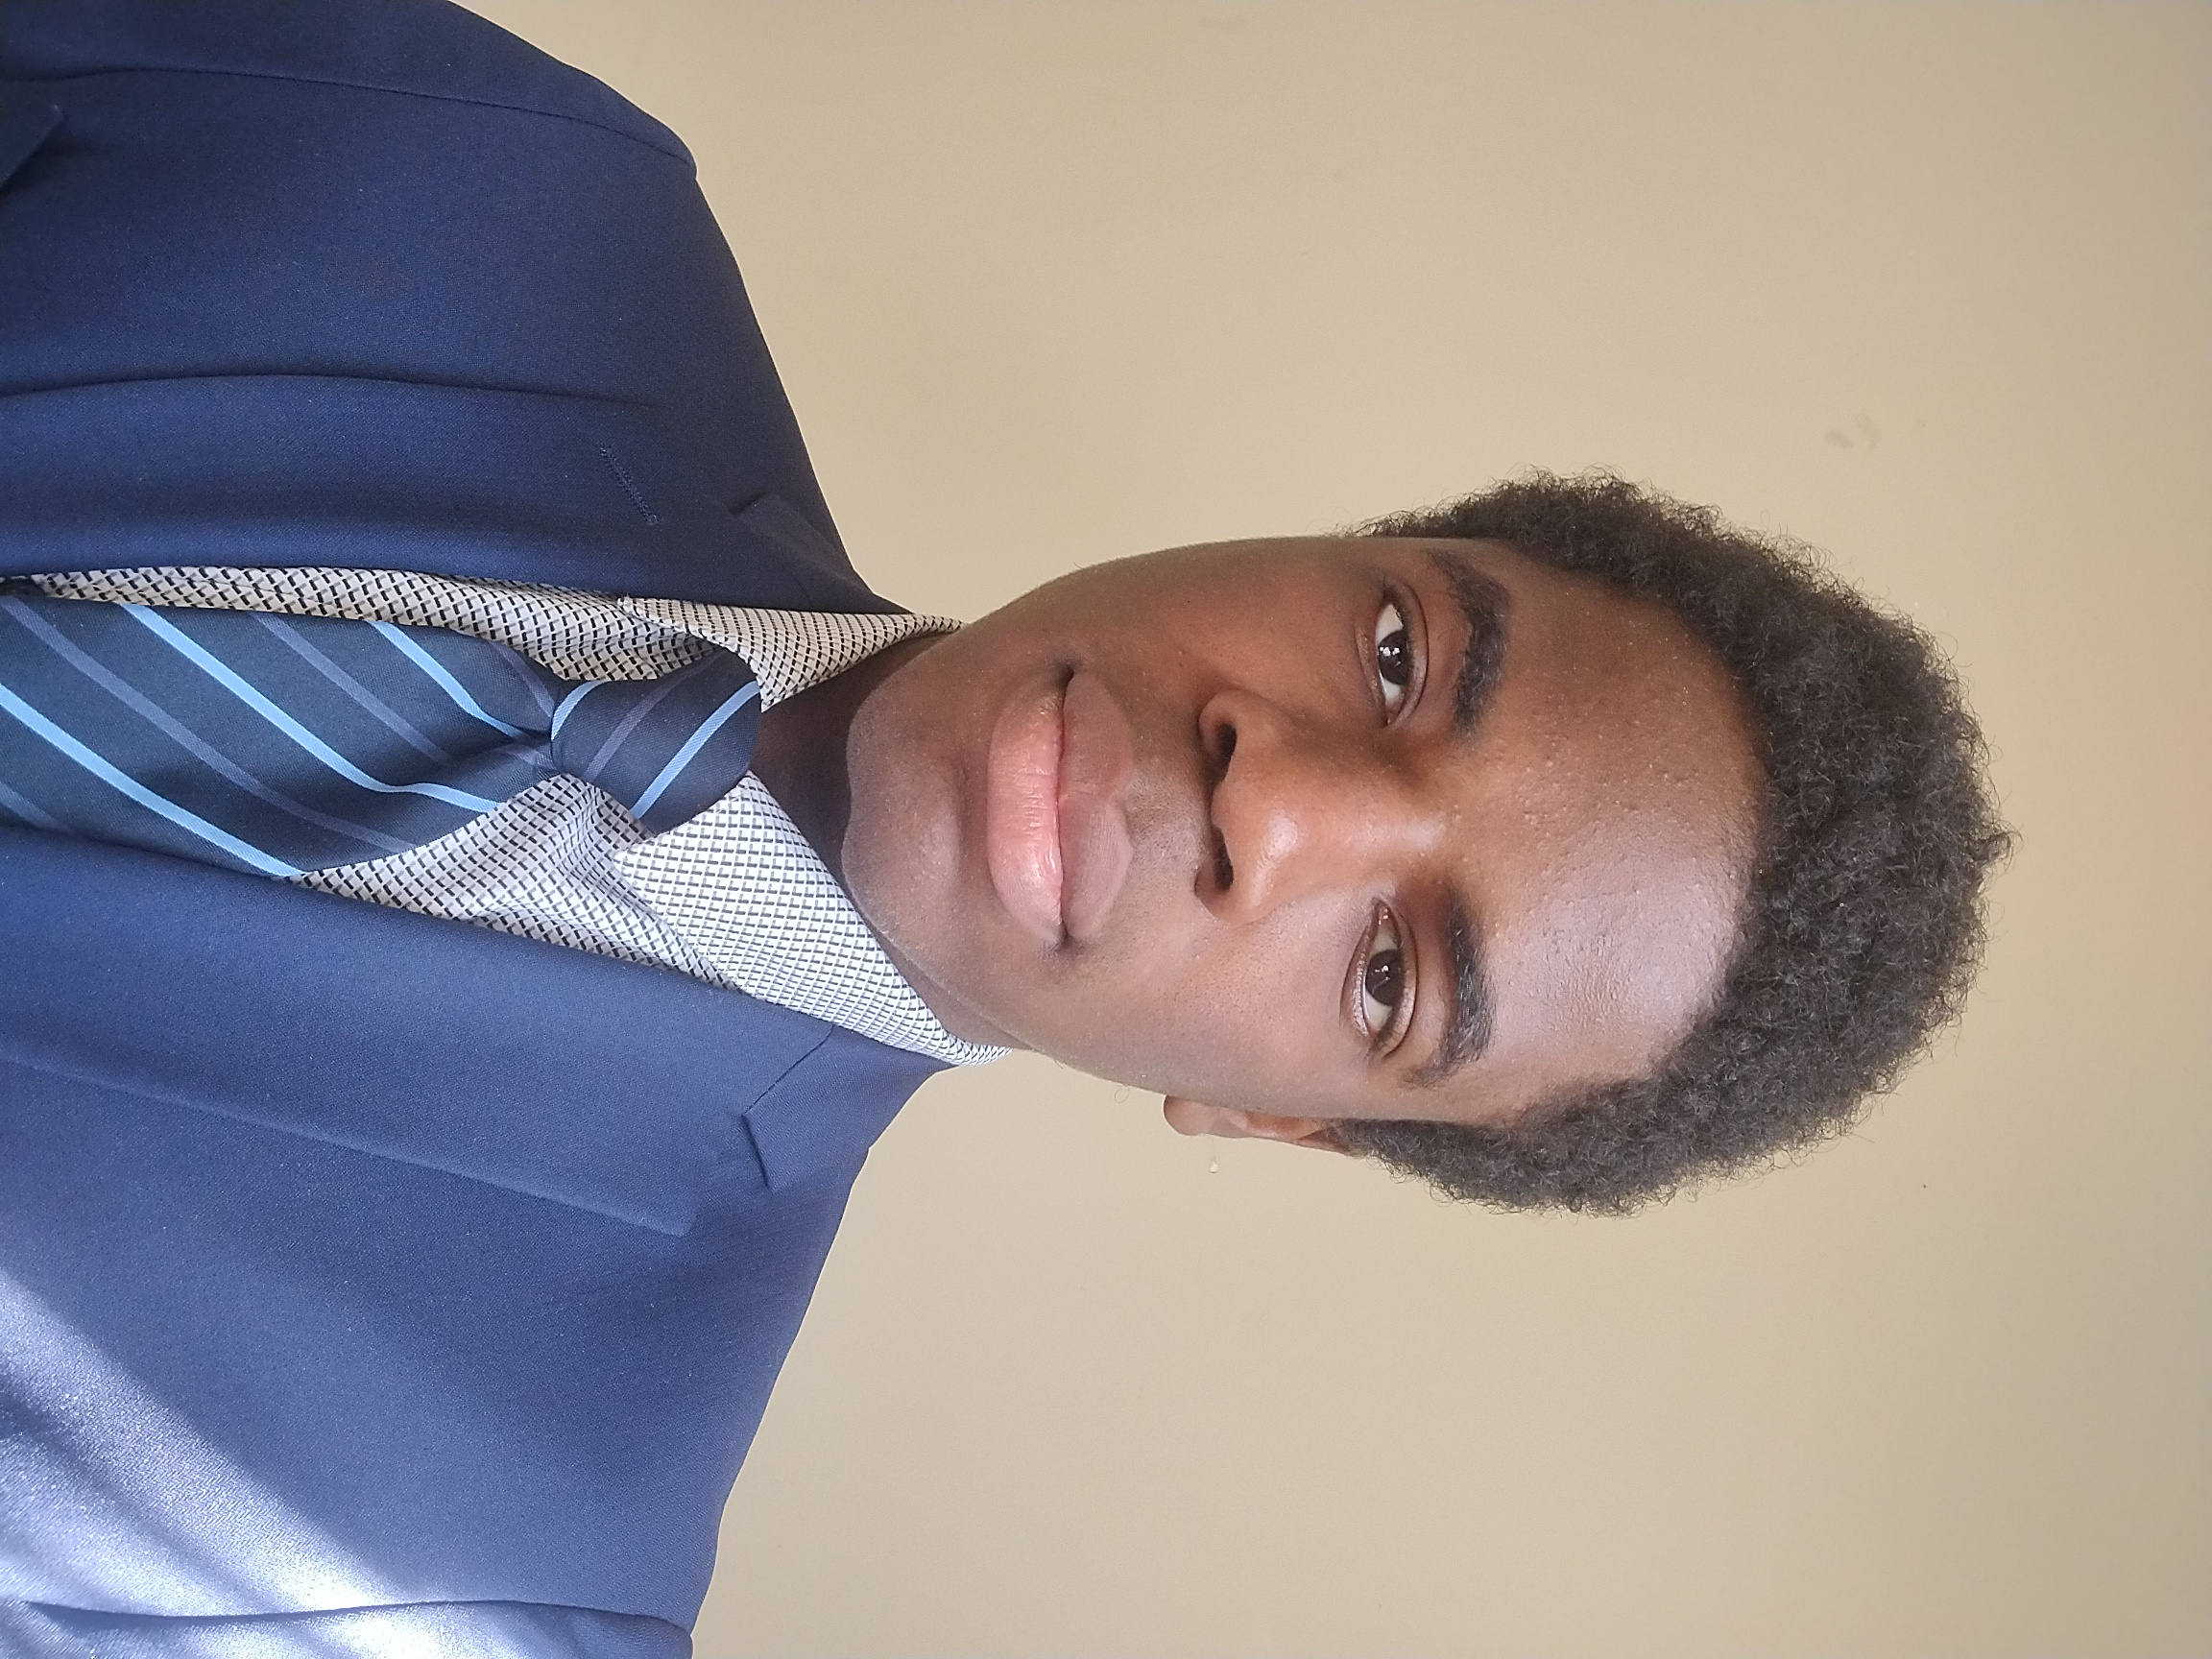
\includegraphics[width=1in,keepaspectratio,angle=90]{../images/mike_odnis.jpg}}]
{Mike Odnis} is enrolled in a Bachelor of Science program in Computer Science, with an anticipated graduation date of May 2026. Demonstrating a strong commitment to ongoing learning and professional growth, his focus is on Full-stack development, along with exploring Machine Learning, Artificial Intelligence, and Software Engineering.
\end{IEEEbiography}
\begin{IEEEbiography}[{
\includegraphics[width=1in,keepaspectratio]{../images/mohammad_alshibli.jpg}}]{Mohammad Alshibli} received his bachelor's degree in Computer Science at Philadelphia University in 2002, his Master of Science degree in Computer Science in 2011 at the Al-Balq’a Applied University, and his Ph.D. in Computer Science and Engineering program at the University of Bridgeport, USA in 2018. His research focuses on decision support techniques, disassembly sequencing, industrial robots, multiple criteria decision-making, robotic manipulation, and metaheuristics. He published his findings in various academic journals and presented his research work in several academic settings. (email: mohammad.alshibli@farmingdale.edu)
\end{IEEEbiography}

\end{document}
